\documentclass[twoside,10pt]{article}
\usepackage{amsmath,amsfonts,amsthm,fullpage}
\usepackage{mymath}
\usepackage{algorithm}
\usepackage{algorithmic}
\usepackage{graphicx}


\begin{document}

\title{CS 7641 CSE/ISYE 6740 Homework 1}
\author{Le Song}
\date{Deadline: 10/9 Thr, 11:59pm}
\maketitle

\begin{itemize}
  \item Submit your answers as an electronic copy on T-square.
  \item No unapproved extension of deadline is allowed. Zero credit will be assigned for late submissions. Email request for late submission may not be replied.
  \item For typed answers with LaTeX (recommended) or word processors, extra credits will be given. If you handwrite, try to be clear as much as possible. No credit may be given to unreadable handwriting.
  \item Explicitly mention your collaborators if any.
  \item Recommended reading: PRML\footnote{Christopher M. Bishop, Pattern Recognition and Machine
Learning, 2006, Springer.} Section 9.1, 12.1
\end{itemize}

%----------------------------------------------------------------------------------
\section{Probability [15 pts]}

\subsubsection*{(a) Stores A, B, and C have 50, 75, and 100 employees and, respectively, 50, 60, and 70 percent of these are women. Resignations are equally likely among all employees, regardless of stores and sex. Suppose an employee resigned, and this was a woman. What is the probability that she has worked in store C? [5 pts]}
 Let W be an Event that a Womenwhich will be probability of resignation as it is equally likely.\\[.25cm]
Let A,B,C be  the Stores.\\[.25cm]
We have to find probability that the employee is from C given employee is a woman
P(C/W) = P(W/C)P(C)/P(W)

$$
P(W/C) = .7,
P(C) = 100/225=.44,
P(W) = P(W/C)P(C) + P(W/B)P(B) + P(W/A)P(A) 
$$
$$
P(W)=  140/225
$$
Putting the values, we get the posterior probability as  \\
P(C/W) = 1/2 = .5\\[.55cm]

\subsubsection*{(b) A laboratory blood test is 95 percent effective in detecting a certain disease when it is, in fact, present. The test also yields a false positive result for 1 percent of the healthy persons tested. That is, if a healthy person is tested then with probability 0.01 the test result will imply he has the disease. If 0.5 percent of the population actually has the disease, what is the probability a person has the disease given that his test result is positive? [5 pts]}
 Let P be an Event that a test shows a disease.\\[.25cm]
Let D be probability that patient has disease.\\[.25cm]
We have to find probability that the person haresult is positives disease given 
P(D/P) = P(P/D)P(D)/P(P)

$$
P(P/D) = .95,
P(P/\neg D) = .01
P(D) = .005,
P(\neg D) = .995,
P(P) = P(P/D)P(D) + P(W/\neg D)P(\neg D) 
$$
$$
P(P)=  .0147
$$
Putting the values \\
P(D/P) = .3231\\[.55cm]
\textbf{[c-d]} On the morning of September 31, 1982, the won-lost records of the three leading baseball teams in the western division of the National League of the United States were as follows:

\begin{table}[!h]
\centering \small
\begin{tabular}{l|c|c}
  \hline
  Team & Won & Lost\\
  \hline \hline
  Atlanta Braves & 87 & 72\\
  San Francisco Giants & 86 & 73\\
  Los Angeles Dodgers & 86 & 73\\
  \hline
\end{tabular}
\end{table}

Each team had 3 games remaining to be played. All 3 of the Giants games were with the Dodgers, and the 3 remaining games of the Braves were against the San Diego Padres. Suppose that the outcomes of all remaining games are independent and each game is equally likely to be won by either participant. If two teams tie for first place, they have a playoff game, which each team has an equal chance of winning.

\subsubsection*{(c) What is the probability that Atlanta Braves wins the division? [2 pts]}
There will be 4 cases when Atlanta wins the division\\
Atlanta wins 3 \\
Atlanta wins 2\\
Atlanta wins 1\\
Atlanta wins 0\\[.30cm]
It should be noted that matches of Atlanta (A) and those between  San Francisco Giants (S) \\
 and  Los Angeles Dodgers(L) are independent events. Thus probablity of these two events is product of indiviual probabilities.\\
 When he wins 3 games then they will be the winner irrespectible of other results.\\
$
P(3wins) = 1/8 \\
$
When he wins 2 games then there are  4 cases(A,S,L) - (2 1 2) , (2 2 1) ,(2 0 3) ,(2 3 0) . In first two cases they win directly and in the last two game will go to\\ playoffs, thus P(2wins) = 3/8(3/8 + 3/8+1/8*1/2+1/8*1/2) = 21/64\\
When he wins 1 game then there are 4 cases (1 1 2) , (1 2 1) ,(1 0 3) ,(1 3 0) . In first two cases it will go to playoffs and in last 2 atlanta loses . \\
$
P(1win) = 3/8*(3/8*1/2 + 3/8*1/2)= 9/64
$
Thus, probability of  Atlanta winning the division is \\ $ P(3wins) +  P(2wins)+P(1win) = 8+21+9/64 = 19/32
$
\subsubsection*{(d) What is the probability to have an additional playoff game? [3 pts]}
There will be 4 cases when Atlanta wins the division\\
Atlanta wins 3 \\
Atlanta wins 2\\
Atlanta wins 1\\
Atlanta wins 0\\
Again we will use the same concept. \\
There will be play offs in the following four cases
 16 cases only when (A S L) is ( 2 0 3 ) (2 3 0)  (1 1 2) (1 2 1) game goes in playoff \\ 
Thus probability of playoff is $$3/8(1/8) +  3/8(1/8) +  3/8(3/8)  +  3/8(3/8) = 3/8$$
%\vspace{1cm}
\newpage

%----------------------------------------------------------------------------------
\section{Maximum Likelihood [15 pts]}

Suppose we have $n$ i.i.d (independent and identically distributed)
data samples from the following probability distribution. This
problem asks you to build a log-likelihood function, and find the
maximum likelihood estimator of the parameter(s).

\subsubsection*{(a) Poisson distribution [5 pts]}
The Poisson distribution is defined as
\begin{equation} \nonumber
P(x_i = k) = \frac{\lambda^k e^{-\lambda}}{k!} (k = 0, 1, 2, ...).
\end{equation}
What is the maximum likelihood estimator of $\lambda$?
  
For n iid data samples, Maximum likelihood is given by :
\begin{equation} \nonumber
L(x) = \prod_{k=1}^{n} P(x_k)  =  \prod_{k=1}^{n} \frac{\lambda^{x_i} e^{-\lambda}}{x_i!} (k = 0, 1, 2, ...).
\end{equation}
\begin{equation} \nonumber
= \frac{\lambda^{\sum x_i}e^{-n \lambda}}{x_1! x_2! ... x_n!}
\end{equation}
$
\log L(x)  =   {\sum x_i} \log \lambda - n\lambda -log {x_1! x_2! ... x_n!} \\[.55cm]
\frac{\partial log L}{d\lambda}  = {\sum x_i}\frac{1}{\lambda} -n = 0 \\ [.55cm]
\lambda = \frac {\sum x_i} {n} \\[.55cm]
$
\subsubsection*{(b) Multinomial distribution [5 pts]}
The probability density function of Multinomial distribution is given by 
$$f(x_1,x_2,\dots,x_k;n,\theta_1,\theta_2,\dots,\theta_k)=\frac{n!}{x_1!x_2!\cdots x_k!}\prod_{j=1}^{k}\theta_j^{x_j},$$
where $\sum_{j=1}^k\theta_j=1,\sum_{j=1}^k x_j=n$. What is the maximum likelihood estimator of $\theta_j, j=1,\dots k$?

For N iid data samples, Maximum likelihood is given by :
\begin{equation} \nonumber
L(x) = \prod_{n=1}^{N} P(x_n)  =\prod_{n=1}^{N}  (\frac{n!}{x_1!x_2!\cdots x_k!}\prod_{j=1}^{k}\theta_j^{x_j})
\end{equation}
\begin{equation} \nonumber
=\frac{n!^N}{(x_1!x_2!\cdots x_k!)^N} \prod_{n=1}^{N}\prod_{j=1}^{k}\theta_j^{x_j}
\end{equation}
\begin{equation} \nonumber
=\frac{n!^N}{(x_1!x_2!\cdots x_k!)^N}\prod_{j=1}^{k}\theta_j^{\sum^{N} x_j}
\end{equation}
Taking the log we get ,(ignoring the constants)
\begin{equation} \nonumber
\log L(x) =\sum_{j=1}^{k}(\sum_{n=1}^{N} x_j  \log\theta_j) 
\end{equation}
We need to maximise $ \log L(x) $ with respect to  $\theta_j $ taking account of constraint  
 $\sum_{j=1}^k\theta_j=1$ \\
\begin{equation} \nonumber
\log L(x) =\sum_{j=1}^{k}(\sum_{n=1}^{N} x_j  \log\theta_j) - \lambda (\sum_{j=1}^k\theta_j-1)
\end{equation}
Setting the derivative with respect to $\theta_j$ , we get 
\begin{equation} \nonumber
\frac{\sum_{n=1}^{N} x_{nj}}{\theta_j} -  \lambda  = 0 
\end{equation}
\begin{equation} \nonumber
\frac{\sum_{n=1}^{N} x_{nj}}{ \lambda} = {\theta_j}  
\end{equation}
Let $ \sum_{n=1}^{N} x_{nj} $ be $ E_j $

\begin{equation} \nonumber
\frac{E_j}{ \lambda} = {\theta_j}  
\end{equation}
Back substituting , and putting the value in constraint, we get
\begin{equation} \nonumber
\sum_{j=1}^k \frac{E_j}{ \lambda} =1 
\end{equation}
thus, $\lambda = n $  as summation of $E_j$  is n, Therefore\\ 
\begin{equation} \nonumber
 \theta_j = \frac {E_j} {n} 
\end{equation}
\subsubsection*{(c) Gaussian normal distribution [5 pts]}
Suppose we have $n$ i.i.d (Independent and Identically Distributed)
data samples from a univariate Gaussian normal distribution
$\mathcal{N}(\mu, \sigma^2)$, which is given by
\begin{equation}
\mathcal{N}(x; \mu, \sigma^2) = \frac{1}{\sigma \sqrt{2\pi}} \exp
\left( - \frac{(x - \mu)^2}{2\sigma^2} \right).\nonumber
\end{equation}
What is the maximum likelihood estimator of $\mu$ and $\sigma^2$?
\begin{equation}
\mathcal{L}(x; \mu, \sigma^2) = \log \prod_{i=1}^n \frac{1}{\sigma \sqrt{2\pi}} \exp
\left( - \frac{(x - \mu)^2}{2\sigma^2} \right).\nonumber
\end{equation}

\begin{equation}
\mathcal{L}(x; \mu, \sigma^2) = -\frac{n}{2}\log 2\pi   -\frac{n}{2}\log \sigma^2 - \sum_{i=1}^n  \frac{(x^i - \mu)^2}{2\sigma^2}.\nonumber
\end{equation}
Taking derivative wrt to u and setting to 0
\begin{equation}
\frac{\partial L}{\partial \mu} = \sum_{i=1}^n  \frac{(x^i - \mu)}{2\sigma^2} = 0.\nonumber
\end{equation}
\begin{equation}
 \mu =\frac{ \sum_{i=1}^n (x^i )}{n} .\nonumber
\end{equation}
Taking derivative wrt to $\sigma^2$ and setting to 0
\begin{equation}
\frac{\partial L}{\partial\sigma^2} =-\frac{m}{\sigma^2} + \frac{1}{2\sigma^4}  \sum_{i=1}^n (x^i - \mu)^2 = 0\nonumber
\end{equation}
\begin{equation}
\sigma^2 =\frac{1}{m}\sum_{i=1}^n (x^i - \mu)^2\nonumber
\end{equation}
\vspace{1cm}




\iffalse
\subsubsection*{(b) Exponential distribution [5 pts]}
The probability density function of Exponential distribution is
given by
\begin{equation} \nonumber
f(x) = \left\{\begin{matrix}
\lambda e^{-\lambda x} & x \ge 0\\
0 & x < 0
\end{matrix}\right.
\end{equation}
What is the maximum likelihood estimator of $\lambda$?
\fi

%----------------------------------------------------------------------------------
\section{Principal Component Analysis [20 pts]}
In class, we learned that Principal Component Analysis (PCA)
preserves variance as much as possible. We are going to explore
another way of deriving it: minimizing reconstruction error.

Consider data points $\text x^n (n=1, ..., N)$ in $D$-dimensional space.
We are going to represent them in $\{\text u_1, ..., \text u_D\}$ orthonormal basis.
That is,
\begin{equation} \nonumber
\text x^n = \sum_{i=1}^D \alpha_i^n \text u_i = \sum_{i=1}^D ({\text x^n}^T \text u_i) \text u_i.
\end{equation}
Here, $\alpha^n_i$ is the length when $\text x^n$ is projected onto
$u_i$.

Suppose we want to reduce the dimension from $D$ to $M < D$. Then
the data point $\text x^n$ is approximated by
\begin{equation} \nonumber
\tilde{\text x}^n = \sum_{i=1}^M z_i^n \text u_i + \sum_{i=M+1}^D b_i \text u_i.
\end{equation}
In this representation, the first $M$ directions of $\text u_i$ are
allowed to have different coefficient $z^n_i$ for each data point,
while the rest has a constant coefficient $b_i$. As long as it is
the same value for all data points, it does not need to be 0.

Our goal is setting $\text u_i$, $z^n_i$, and $b_i$ for $n = 1,..., N$
and $i = 1, ..., D$ so as to minimize reconstruction error. That is,
we want to minimize the difference between $\text x^n$ and $\tilde{\text x}^n$ over $\{ \text u_i, z^n_i, b_i \}$:
\begin{equation} \nonumber
J = \frac{1}{N} \sum_{n=1}^N \| \text x^n - \tilde{\text x}^n \|^2.
\end{equation}
\subsubsection*{(a) What is the assignment of $z_j^n$ for $j=1, ..., M$ minimizing $J$? [5 pts]}

Putting the values for J, we get \\
$$
J = \frac{1}{N} \sum_{n=1}^N \| \text x^n - \sum_{i=1}^M z_i^n \text u_i + \sum_{i=M+1}^D b_i \text u_i \|^2 \\
$$
We know that for
 $$
L = \|xu\|^2
 $$

 $$
\frac{ \partial L }{ \partial x} = 2 u^T.(xu) 
$$
Thus, we will get the following equation. We got rid of summation as it is wrt to single point n. \\[.20cm]
$$\frac{\partial J}{\partial z^n_i} =(u_i)^T .(\frac{1}{N} \sum_{n=1}^N  \text x^n - \sum_{i=1}^M z_i^n \text u_i + \sum_{i=M+1}^D b_i \text u_i) 
$$
Since, this is a scalar, we can take its transpose and setting it to 0
$$\frac{\partial J}{\partial z^n_i} = \frac{2}{N} ((x^n)^T - \sum_{i=1}^M z_i^n u_i^T + \sum_{i=M+1}^D b_i u_i^T).(u_i) = 0
$$

From orthonormality condition $u_i^T.u_j = \delta_{ij}$  which is equal to one when i  is equal to j and zero otherwise, we get

\begin{equation} \nonumber
\begin{split}
\frac{\partial J}{\partial z^n_i} = \frac{2}{N} (-(x^n)^T.(u_i) + z_i^n) = 0
\end{split}
\end{equation}

After equating this to 0, we get,

\begin{equation} \nonumber
\begin{split}
(-(x^n)^T.(u_i) + z_i^n) = 0\\
z_i^n = (x^n)^T.(u_i)
\end{split}
\end{equation}

\subsubsection*{(b) What is the assignment of $b_j$ for $j=M+1, ..., D$ minimizing $J$? [5 pts]}
Similarly to how we did in last part, \\
\begin{equation} \nonumber
\begin{split}
J = \frac{1}{N} \sum_{n=1}^N \| \text x^n - \sum_{i=1}^M z_i^n \text u_i + \sum_{i=M+1}^D b_i \text u_i \|^2 \\
\frac{\partial J}{\partial b_i} = \frac{2}{N} \sum_{n=1}^N ((x^n)^T - \sum_{i=1}^M z_i^n u_i^T + \sum_{i=M+1}^D b_i u_i^T).(u_i)
\end{split}
\end{equation}


From orthonormality condition $u_i^T.u_j = \delta_{ij}$  which is equal to one when i  is equal to j and zero otherwise, we get

\begin{equation} \nonumber
\begin{split}
\frac{\partial J}{\partial b_i} = \frac{2}{N} \sum_{n=1}^N ((x^n)^T.(u_i) - b_i) =0
\end{split}
\end{equation}

\begin{equation} \nonumber
\begin{split}
\sum_{n=1}^N (-(x^n)^T.(u_i) + b_i) &= 0\\
b_i &= \frac{\sum_{n=1}^N (x^n)^T}{N}.(u_i)\\
b_i &= \bar{x}^T.u_i
\end{split}
\end{equation}

\subsubsection*{(c) Express optimal $\tilde{\text x}^n$ and $\text x^n - \tilde{\text x}^n$ using your answer for (a) and (b). [2 pts]}

\begin{equation} \nonumber
\begin{split}
\tilde{\text x}^n &= \sum_{i=1}^M z_i^n \text u_i + \sum_{i=M+1}^D b_i \text u_i \\
&= \sum_{i=1}^M ((x^n)^T.(u_i)) \text u_i + \sum_{i=M+1}^D (\bar{x}^T.u_i) \text u_i
\end{split}
\end{equation}

\begin{equation} \nonumber
\begin{split}
\text x^n - \tilde{\text x}^n &= \sum_{i=1}^D ({\text x^n}^T \text u_i) \text u_i - \sum_{i=1}^M z_i^n \text u_i - \sum_{i=M+1}^D b_i \text u_i \\
&= \sum_{i=M+1}^D ((x^n)^T.(u_i)) \text u_i - \sum_{i=M+1}^D (\bar{x}^T.u_i) \text u_i \\
&= \sum_{i=M+1}^D \{(x^n - \bar{x})^T u_i\} u_i
\end{split}
\end{equation}

\subsubsection*{(d) What should be the $\text u_i$ for $i=1, ..., D$ to minimize $J$? [8 pts]}

\begin{equation} \nonumber
\begin{split}
J &= \frac{1}{N} \sum_{n=1}^N \| \text x^n - \tilde{\text x}^n \|^2 \\
J &= \frac{1}{N} \sum_{n=1}^N \| \sum_{i=M+1}^D \{u_i^T (x^n - \bar{x})\} u_i \|^2 \\
J &= \frac{1}{N} \sum_{n=1}^N \sum_{i=M+1}^D (\{u_i^T (x^n - \bar{x})\} u_i)(\{u_i^T (x^n - \bar{x})\} u_i)^T \\
J &= \frac{1}{N} \sum_{n=1}^N \sum_{i=M+1}^D (\{u_i^T (x^n - \bar{x})\} u_i)( u_i^T \{(x^{nT} - \bar{x}^T)u_i\})
\end{split}
\end{equation}

Now using the orthonormality condition $u_i^T.u_j = \delta_{ij}$, we get:

\begin{equation} \nonumber
\begin{split}
J &= \frac{1}{N} \sum_{n=1}^N \sum_{i=M+1}^D (\{u_i^T(x^{n} - \bar{x})\})(\{(x^{nT} - \bar{x}^T)u_i\}) \\
\end{split}
\end{equation}
$
= \frac{1}{N} \sum_{n=1}^N \sum_{i=M+1}^D (u_i^T x^{n} - u_i^T \bar{x})(x^{nT} u_i - \bar{x}^T u_i) \\
= \frac{1}{N} \sum_{n=1}^N \sum_{i=M+1}^D (u_i^T x^{n} x^{nT} u_i - u_i^T \bar{x} x^{nT} u_i - u_i^T x^{n} \bar{x}^T u_i + u_i^T \bar{x} \bar{x}^T u_i) \\
= \frac{1}{N} \sum_{n=1}^N \sum_{i=M+1}^D u_i^T (x^{n} x^{nT} - \bar{x} x^{nT} - x^{n} \bar{x}^T + \bar{x} \bar{x}^T u_i) u_i \\
= \frac{1}{N} \sum_{n=1}^N \sum_{i=M+1}^D u_i^T (\text x^n - \bar{\text x})(\text x^n - \bar{\text x})^T u_i \\
= \sum_{i=M+1}^D u_i^T (\frac{1}{N} \sum_{n=1}^N (\text x^n - \bar{\text x})(\text x^n - \bar{\text x})^T) u_i \\ 
= \sum_{i=M+1}^D u_i^T S u_i \\
$
Thus ,
\begin{equation} \nonumber
\begin{split}
J &= \sum_{i=M+1}^D u_i^T S u_i \\
\end{split}
\end{equation}

Now , we need to differentiate   J wrt $u_i$ subjected to constraint  from the orthonormality condition $u_i^T.u_j = \delta_{ij}$ by taking the Lagrange multiplier we get,

\begin{equation} \nonumber
\begin{split}
J_i = u_i^T S u_i + \lambda_i (1 - u_i^T u_i)
\end{split}
\end{equation}

Now, we differentiating J with respect to $u_i$:

\begin{equation} \nonumber
\begin{split}
\frac{\partial J_i}{\partial u_i} = S u_i - \lambda_i u_i
\end{split}
\end{equation}

Setting this to zero, we get:

\begin{equation} \nonumber
\begin{split}
S u_i = \lambda_i u_i, i = 1, ... , D 
\end{split}
\end{equation}

Thus, the corresponding value of the distortion measure is:

\begin{equation} \nonumber
\begin{split}
J &= \sum_{i=M+1}^D u_i^T S u_i \\
J &= \sum_{i=M+1}^D \lambda_i
\end{split}
\end{equation}

\emph{Hint:} Use $S = \frac{1}{N} \sum_{n=1}^N (\text x^n - \bar{\text x})(\text x^n -
\bar{\text x})^T$ for sample covariance matrix. \vspace{1cm}


%----------------------------------------------------------------------------------
\section{Clustering [20 pts]}

\textbf{[a-b]} Given $N$ data points $\text x^n (n=1,\dots,N)$, $K$-means clustering algorithm groups them into $K$ clusters by minimizing the distortion function over $\{ r^{nk}, \mu^k \}$
$$J=\sum_{n=1}^N\sum_{k=1}^Kr^{nk} \|\text x^n-\mu^k\|^2,$$
where $r^{nk}=1$ if $\text x^n$ belongs to the $k$-th cluster and $r^{nk}=0$ otherwise.

\subsubsection*{(a) Prove that using the squared Euclidean distance $\|\text x^n-\mu^k\|^2$ as the dissimilarity function and minimizing the distortion function, we will have 
   $$\mu^k=\frac{\sum_n r^{nk} \text x_n}{\sum_n r^{nk}}.$$
   That is, $\mu^k$ is the center of $k$-th cluster. [5 pts]}
 We can write J as 
$$J=\sum_{n=1}^N\sum_{k=1}^Kr^{nk} (\text x^n-\mu^k)^T (\text x^n-\mu^k),$$
Taking the derivative wrt to $u^k$
$$ \bigtriangledown_{u^k} J=\sum_{n=1}^N r^{nk}(-2x^n + 2 u^k) = 0$$

Thus, \\
\begin{equation}
u^k=\frac{\sum_{n=1}^N r^{nk}(x^n) }{\sum_{n=1}^N r^{nk}}\nonumber
\end{equation}
\subsubsection*{(b) Prove that $K$-means algorithm converges to a local optimum in finite steps. [5 pts]}
To check it converges to optimum, we need to check if it comes to global minimum. So we take derivative for gradient again wrt to k th component/vector of j
$$ \frac{ \partial{  \bigtriangledown_{u^k}J}}{d(u^{jk})} = \frac{d }{d(u^{jk})}\sum_{n=1}^N r^{nk}(-2x^n + 2 u^k) =2({\sum_{n=1}^N r^{nk}})I >0$$
 Now , $r^{nk}$ values can be 0 or 1. So, it is basically number of points assigned to k. This will be positive definate as long as 1 point is assigned to k. \\ Incase, there is no point assigned to k , then we remove that center. \\[.55cm]

Inituitively, we can say that as long as we have k clusters , k means try to decrease cost function, till the time contribution towards cost for a particular cluster becomes minimum. \\[.25cm]
\textbf{[c-d]} In class, we discussed bottom-up hierarchical clustering. For each iteration, we need to find two clusters $\{\text x_1, \text x_2, \dots, \text x_m\}$ and $\{\text y_1, \text y_2, \dots, \text y_p\}$ with the minimum distance to merge. Some of the most commonly used distance metrics between two clusters are:
    \begin{itemize}
    \item Single linkage: the minimum distance between any pairs of points from the two clusters, i.e.
    $$\min_{i=1,\dots,m \atop j=1,\dots, p}\|\text x_i - \text y_j\|$$
    \item Complete linkage: the maximum distance between any parts of points from the two clusters, i.e.
    $$\max_{i=1,\dots,m \atop j=1,\dots, p}\|\text x_i - \text y_j\|$$
    \item Average linkage: the average distance between all pair of points from the two clusters, i.e.
    $$\frac{1}{mp}\sum_{i=1}^m\sum_{j=1}^p\|\text x_i - \text y_j\|$$
    \end{itemize}

\subsubsection*{(c) When we use the bottom up hierarchical clustering to realize the partition of data, which of the three cluster distance metrics described above would most likely result in clusters most similar to those given by $K$-means? (Suppose $K$ is a power of 2 in this case). [5 pts]}

In Bottom up hierarchy, we combine to clusters which have the minimum distance to merge.  I believe that Average Linkage is most likely to get us clusters similar to K means. The reason is because as we select center in K means which is basically average of all points, which helps in reducing the impact of extreme points. Similarly  joining clusters in Average Linkage will help in reducing impact of outliers. In case of  minimum, it is possible that lets say we have 3 clusters and out of which, two are relatively close and other is far off, however far has one point very close to one of the clusters , then it will result in far cluster merged with one of the closer cluster. Similarly , in case of maximum, it is possible that two clusters are really closer , however there exists one point in either one which is very far/outlier. This will to result in further cluster merged  with one of the two closer ones .  However average will tend to decrease the effect of outlier as done in the K-means. \\

\subsubsection*{(d) For the following data (two moons), which of these three distance metrics (if any) would successfully separate the two moons? [5 pts]}

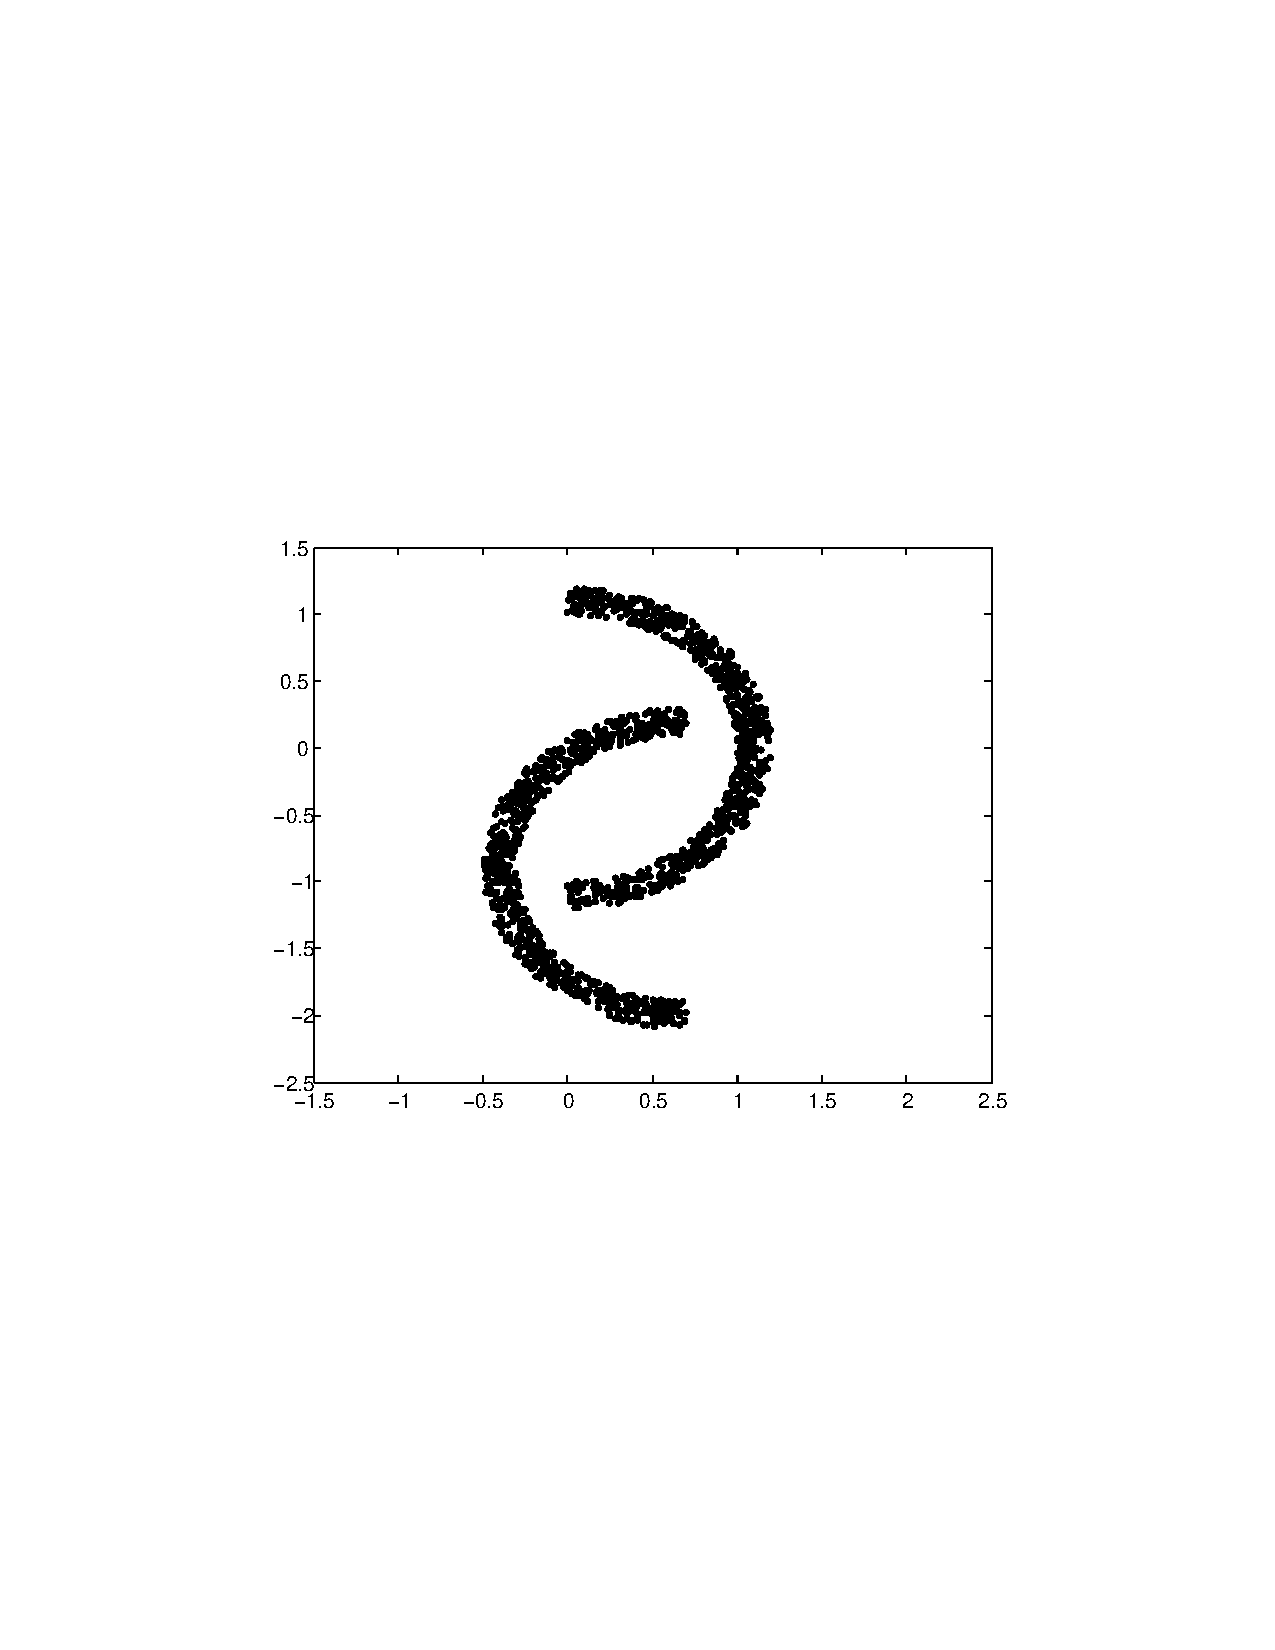
\includegraphics[trim = 0mm 90mm 0mm 90mm, clip, width = \linewidth]{clustering}
Single Linkage (Minimum distance ) will successfully separate the two moons. The reason is that the every time we merge  two clusters, they will look for minimum distance , which will be formed by joining two continuous parts of a single moon. It will not prefer merging across moons as minimum distance between two moons is greater than the two continuous parts of a single moon.( there is minimum distance d between 2 moons which is greater than distance between continuous parts.) 
\vspace{1cm}



%----------------------------------------------------------------------------------
\section{Programming: Image compression [30 pts]}

In this programming assignment, you are going to apply clustering algorithms for image compression. Before starting this assignment, we strongly recommend reading PRML Section 9.1.1, page 428 -- 430.

To ease your implementation, we provide a skeleton code containing image processing part. \texttt{homework1.m} is designed to read an RGB bitmap image file, then cluster pixels with the given number of clusters $K$. It shows converted image only using $K$ colors, each of them with the representative color of centroid. To see what it looks like, you are encouraged to run \texttt{homework1(`beach.bmp', 3)} or \texttt{homework1(`football.bmp', 2)}, for example.

Your task is implementing the clustering parts with two algorithms: \emph{$K$-means} and \emph{$K$-medoids}. We learned and demonstrated $K$-means in class, so you may start from the sample code we distributed.

The file you need to edit is \texttt{mykmeans.m} and \texttt{mykmedoids.m}, provided with this homework. In the files, you can see it calls Matlab function \texttt{kmeans} initially. Comment this line out, and implement your own in the files. You would expect to see similar result with your implementation of $K$-means, instead of \texttt{kmeans} function in Matlab.

\subsubsection*{$K$-medoids}

In class, we learned that the basic $K$-means works in Euclidean space for computing distance between data points as well as for updating centroids by arithmetic mean. Sometimes, however, the dataset may work better with other distance measures. It is sometimes even impossible to compute arithmetic mean if a feature is categorical, e.g, gender or nationality of a person. With $K$-medoids, you choose a representative data point for each cluster instead of computing their average.

Given $N$ data points $\text x^n (n = 1, ..., N)$, $K$-medoids clustering algorithm groups them into $K$ clusters by minimizing the distortion function $J = \sum_{n=1}^N \sum_{k=1}^K r^{nk} D(\text x^n, \mu^k)$,
where $D(\text x, \text y)$ is a distance measure between two vectors $\text x$ and $\text y$ in same size (in case of $K$-means, $D(x, y) = \| \text x - \text y \|^2$), $\mu^k$ is the center of $k$-th cluster; and $r^{nk} = 1$ if $\text x^n$ belongs to the $k$-th cluster and $r^{nk} = 0$ otherwise. In this exercise, we will use the following iterative procedure:

\begin{itemize}
  \item Initialize the cluster center $\mu^k$, $k = 1, ..., K$.
  \item Iterate until convergence:
  \begin{itemize}
    \item Update the cluster assignments for every data point $\text x^n$: $r^{nk} = 1$ if $k = \argmin_j D(\text x^n, \mu^j)$, and $r^{nk} = 0$ otherwise.
    \item Update the center for each cluster $k$: choosing another representative if necessary.
  \end{itemize}
\end{itemize}

There can be many options to implement the procedure; for example, you can try many distance measures in addition to Euclidean distance, and also you can be creative for deciding a better representative of each cluster. We will not restrict these choices in this assignment. You are encouraged to try many distance measures as well as way of choosing representatives.


\subsubsection*{Formatting instruction}

Both \texttt{mykmeans.m} and \texttt{mykmedoids.m} take input and output format as follows. You should not alter this definition, otherwise your submission will print an error, which leads to zero credit.\\

\textbf{Input}
\begin{itemize}
  \item \texttt{pixels}: the input image representation. Each row contains one data point (pixel). For image dataset, it contains 3 columns, each column corresponding to Red, Green, and Blue component. Each component has an integer value between 0 and 255.
  \item \texttt{K}: the number of desired clusters. Too high value of $K$ may result in empty cluster error. Then, you need to reduce it.
\end{itemize}

\textbf{Output}
\begin{itemize}
  \item \texttt{class}: cluster assignment of each data point in pixels. The assignment should be 1, 2, 3, etc. For $K = 5$, for example, each cell of class should be either 1, 2, 3, 4, or 5. The output should be a column vector with \texttt{size(pixels, 1)} elements.
  \item \texttt{centroid}: location of $K$ centroids (or representatives) in your result. With images, each centroid corresponds to the representative color of each cluster. The output should be a matrix with $K$ rows and 3 columns. The range of values should be [0, 255], possibly floating point numbers.
\end{itemize}

\subsubsection*{Hand-in}
Both of your code and report will be evaluated. Upload \texttt{mykmeans.m} and \texttt{mykmedoids.m} files with your implementation. In your report, answer to the following questions:
\begin{enumerate}
  \item Within the $K$-medoids framework, you have several choices for detailed implementation. Explain how you designed and implemented details of your $K$-medoids algorithm, including (but not limited to) how you chose representatives of each cluster, what distance measures you tried and chose one, or when you stopped iteration.
  \item Attach a picture of your own. We recommend size of $320 \times 240$ or smaller.
  \item Run your $K$-medoids implementation with the picture you chose above, with several different $K$. (e.g, small values like 2 or 3, large values like 16 or 32) What did you observe with different $K$? How long does it take to converge for each $K$?
  \item Run your $K$-medoids implementation with different initial centroids/representatives. Does it affect final result? Do you see same or different result for each trial with different initial assignments? (We usually randomize initial location of centroids in general. To answer this question, an intentional poor assignment may be useful.)
  \item Repeat question 2 and 3 with $K$-means. Do you see significant difference between $K$-medoids and $K$-means, in terms of output quality, robustness, or running time?
\end{enumerate}




\subsubsection*{Note}
\begin{itemize}
  \item You may see some error message about empty clusters even with Matlab implementation, when you use too large $K$. Your implementation should treat this exception as well. That is, do not terminate even if you have an empty cluster, but use smaller number of clusters in that case.

  \item We will grade using test pictures which are not provided. We recommend you to test your code with several different pictures so that you can detect some problems that might happen occasionally. 

  \item If we detect copy from any other student's code or from the web, you will not be eligible for any credit for the entire homework, not just for the programming part. Also, directly calling Matlab function \texttt{kmeans} or other clustering functions is not allowed.
\end{itemize}


\subsubsection*{Report}
\begin{itemize}
  \item
For k - medoids , I started with the basic implementation of PAM algorithm. However, the general version had  $O(n^2)$ complexity, due to which I had to shift to some kind of heuristics/approximation. My approach was that I wanted to find a point that was  closest to the center. That is the point lying closest to the cluster center. Idea  for using k medoid over k means is to reduce the impact of outliers by taking a point closest to average. Thus even though average might get persuaded by the outlier, but  once we find an point, it is likely to be closer to the true center of the cluster. We took various distance like seuclidean,minkowski, Manhatten. I have taken Manhatten as representative for this image as it even though might give some less optimal clusters but it was giving me sharper/minor features. As even small part of cloud was differntiated in manhatten.
\item
I tried with different number of iterations. Number of iterations was generally dependent on initial points taken to initialise the image. Even if initial points were random, still number of iterations varied for different images. I even varied the epilon(threshold for convergence), which gave different results. Currently, I have kept it at $10^{-4}$ and a maximum of about 20 iterations,  which gave the advantages of both the speed as well as quality.
  \item
In general as K increases , cluster allocation time will increase as we have to check for minimum distance across all the cluster centers. This is true for both K-means and K-medoids. However , the center allocation part would be constant for k means as we are basically taking the mean for all points irrespective of the number of clusters, but in approximate K-medoid as we check the minimum distance between points , so this will also be k times $n/k$, which will again be same for the given data points. However, in the PAM version of K medoid, as the size increased it gave better performance because the number of pair wise distance calculations decreased as it was k times $n^2 /k^2$ , which decreased with increasing k.
\item For both the k means and k medoids , as we went to k=16, 32, it gave very nice featured image but was time intensive because of the initial distance calculation for k centers.
\item This was true for both k-means and k - medoids.Initial points also had an impact in 3 ways. Firstly, if the points were badly chosen,like adjacent ones , then the initial iteration took lot of time. After few it become fast but that initial iterations had big impact on overall time. \\
Secondly, output was also impacted, as when I took equi spaced points they kind of gave better and well defined clusters.\\
Also, sometimes when bad initial centers not only time for intial clusters was impacted, it also took them more number of iterations to converge.\\

Having said this, K medoid was more agnostic of initial points. As even if initial points were outliers in both the case, then K - medoid was able to converge faster and gave better clusters as compared to K-means. K medoid was able to converge in about 15 iterations as compared to 25 iterations for K-means.
So , I have used 15 iterations for K medoids and 25 for k-means. However, it will finish incase they converge before that.

For k values in 3 to 10 k medoid was converging in 18- 20 seconds and k means was converging in about 23- 25 seconds. However with large k(>20), it took around 60 seconds to converge . Here also , K medoids most of of times was faster.
\end{itemize}
%\bibliographystyle{plain}
%\bibliography{temp,externalPapers,groupPapers}

\end{document}
